\documentclass[a4paper]{article}
\usepackage{amsmath,amssymb,caption,float,graphicx,xcolor}
\usepackage{minted}
\usepackage[utf8]{inputenc}
\usepackage[english]{babel}
\usepackage[backend=bibtex]{biblatex}
\addbibresource{Homework6.bib}
\captionsetup[figure]{labelsep=period}
\definecolor{bg}{rgb}{0.95,0.95,0.95}
\renewcommand\thesection{\arabic{section}}
\usemintedstyle{emacs}
\begin{document}
\begin{center}
    \huge
    \textbf{VE482\\Introduction to Operating Systems\\}
    \Large
    \vspace{15pt}
    \uppercase{\textbf{Homework 6}}\\
    \large
    \vspace{5pt}\today\\
    \vspace{5pt}
    Yihua Liu 518021910998
    \vspace{5pt}
    \rule[-5pt]{.97\linewidth}{0.05em}
\end{center}
\section*{Ex. 1 — Simple questions}
\begin{enumerate}
    \item Consider a swapping system in which memory consists of the following hole sizes in memory order: 10 KB, 4 KB, 20 KB, 18 KB, 7 KB, 9 KB, 12 KB, and 15 KB. Assuming first fit is used, which hole is taken for successive segment requests of: (i) 12 KB, (ii) 10 KB and (iii) 9KB. Repeat for best fit and quick fit.\\
    First fit: (i) Take the third hole (20 KB hole); (2) Take the first hole (10 KB hole); (3) Take the fourth hole (18 KB hole).\\
    Best fit: (i) Take the seventh hole (12 KB hole); (2) Take the first hole (10 KB hole); (3) Take the sixth hole (9 KB hole).\\
    Quick fit: (i) Take the seventh hole (12 KB hole); (2) Take the first hole (10 KB hole); (3) Take the sixth hole (9 KB hole).
    \item If an instruction takes 10 nsec and a page fault takes an additional $n$ nsec, give a formula for the effective instruction time if page faults occur every $k$ instructions.\\
    The effective instruction time if page faults occur every $k$ instructions is
    \[10+\frac{n}{k}.\]
    \item A small computer has four page frames. At the first clock tick, the $R$ bits are 0111. At $t$ subsequent clock tics, the values are 1011, 1010, 1101, 0010, 1010, 1100 and 0001. Assuming the aging algorithm is used with an 8-bit counter what is the value of the four counters after the last tick.\\
    \begin{table}[H]
        \centering
        \begin{tabular}{|c|c|c|c|c|c|c|c|c|}
            \hline
            &$t_0$&$t_1$&$t_2$&$t_3$&$t_4$&$t_5$&$t_6$&$t_7$\\
            \hline
            $p_1$&00000000&10000000&11000000&11100000&01110000&10111000&11011100&01101110\\
            \hline
            $p_2$&10000000&01000000&00100000&10010000&01001000&00100100&10010010&01001001\\
            \hline
            $p_3$&10000000&11000000&11100000&01110000&10111000&11011100&01101110&00110111\\
            \hline
            $p_4$&10000000&11000000&01100000&10110000&01011000&00101100&00010110&10001011\\
            \hline
        \end{tabular}
        \caption{Page replacement - Aging}
    \end{table}
    Thus, the values of the four counters after the last tick are 01101110, 01001001, 00110111, and 10001011.
\end{enumerate}
\section*{Ex. 2 — Page tables}
In the lecture it was mentioned that the translation from virtual address into physical address could be speeded up using the TLB. Unfortunately this solution is not of much help in the case of large page tables. Investigate the two following alternative solutions: inverted page tables and multilevel page tables.
\setcounter{section}{2}
\subsection{Multi-level Page Tables}
Multi-level page tables is to "chop up page table into page-size utils". If an entire page of page-table entries (PTEs) is invalid, multi-level page tables do not allocate that page of the page table. Multi-level page tables use a structure called the page directory, which can tell where a page of the page table is or that "the entire page of the page table contains no valid pages".
\begin{figure}[H]
    \centering
    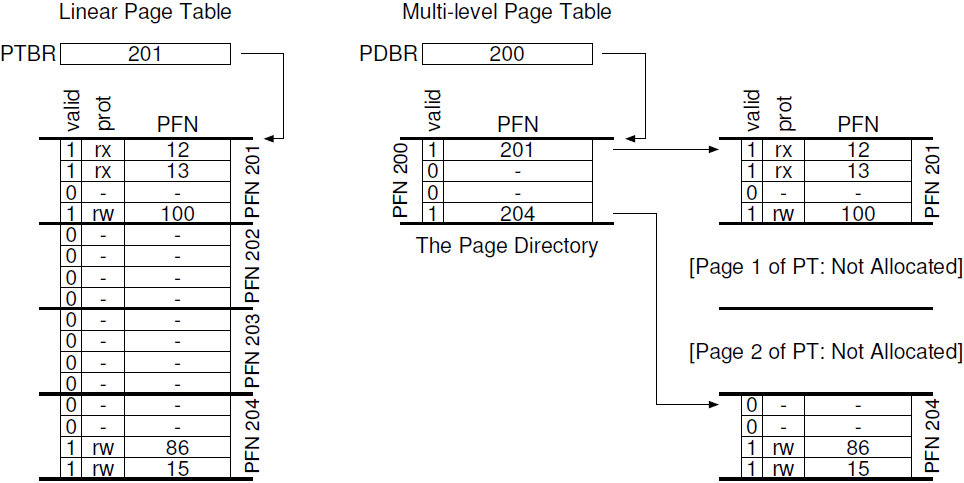
\includegraphics[width=1\textwidth]{2.png}
    \caption{Linear (Left) And Multi-Level (Right) Page Tables \cite{ostep}.}
\end{figure}
Take two-level table as an example, the page directory contains a number of page directory entries (PDE), which includes a valid bit and a page frame number (PFN). If a PDE is valid, through PFN, at least one of the pages of the page table is valid, otherwise, the rest of the PDE is not defined \cite{ostep}.

Compared with linear page tables, multi-level page tables can allocate space in proportion to the address space in use, so that the page tables are more compact. Besides, it is easier to manage memory because every part of a page table can be neatly put in one page. However, this method is complex and is a trade-off between time and space.
\subsection{Inverted Page Tables}
In inverted page tables, weonly reserve one page table that "has an entry for each physical page of the system rather than many page tables and each one for one system process \cite{ostep}. The PTE indicates process that is using this page and the process's virtual page that the process maps to the physical page.
\begin{figure}[H]
    \centering
    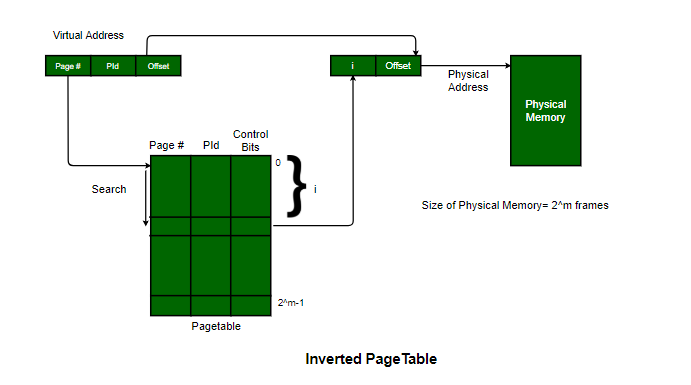
\includegraphics[width=1\textwidth]{3.png}
    \caption{Inverted Page Tables \cite{ipt}.}
\end{figure}
To find the correct entry is just to search through the data structure. The data structure can be a hash table to reduce time costs. The data structure generally consists of a page table and a frame table, one row of the page table corresponds to one frame. Each row has a virtual page number entry, a physical page number entry, etc.

The problem of this method is that the hash function reduce cache spatial locality.
\section*{Ex. 3 — Research}
\begin{enumerate}
    \item Write about half a page on the topic of codes bugs that lead to security holes; in particular illustrate the discussion using common examples. Do not forget to reference your sources of information.\\
    Security holes are vulnerabilities problems of programs. Many faults may lead to security holes. One of the most famous security hole is the buffer overflow. Among different programming languages, C language lacks boundary checks of the memory, and its standard library contains some dangerous functions that may cause buffer overflow if wrongly used \cite{enwiki:1055115654}. For example,
    \begin{minted}[frame=single,bgcolor=bg,breaklines,linenos]{c}
#include <stdio.h>
#include <string.h>

int main() {
    char str[3];
    strcpy(str, "too_many_characters");
    return 0;
}
    \end{minted}
    If a malevolent attacker uses this buffer flow to run a shell and then execute other commands, the system may be hacked.\\
    Another example is format string attacks. An example from CWE-134 is provided here \cite{fmtstr}:
    \begin{minted}[frame=single,bgcolor=bg,breaklines,linenos]{c}
#include <stdio.h>
#include <string.h>

void printWrapper(char *string) {
    printf("%s", string);
}

int main(int argc, char **argv) {
    char buf[5012];
    memcpy(buf, argv[1], 5012);
    printWrapper(argv[1]);
    return (0);
}
    \end{minted}
    The problem is C cannot know if how many arguments there are, so function like \texttt{printf()} can be used to print arbitrary amount of information from the stack. A malevolent attacker can expose the data on the stack or even inject data onto the stack.
    \item Explain what Meltdown and Spectre are. Focus on the hardware and OS part of those attacks. Also explain the idea behind the fixes.\\
    Meltdown is to break the isolation between the operating system and user applications, which allows a program to access the memory so that a program can access secrets of other programs or the operating system. On the other hand, Spectre breaks the isolation between different applications. It is harder to exploit but also harder to mitigate, as more safety checks may increase the risk of being attacks \cite{meltdownattack}.\\
    Meltdown makes use of the side-effects of out-of-order execution on modern processors. It can read arbitrary memory locations, including secure data and passphrases. Briefly, meltdown attackers let the CPU to execute a transient instruction sequence which "uses an inaccessible secret value stored somewhere in physical memory" and "acts as the transmitter of a covert channel" ultimately leaking the secret value to the attacker \cite{Lipp2018meltdown}.\\
    Firstly, the content of a memory location chosen by the attacker but is inaccessible to the attacker is loaded into a register. Secondly, a transient instruction accesses a cache line based on the register's secret content. Finally, the attackers flush and reload to determine the accessed cache line, so that the secret stored at the memory location chosen by the attacker can be retrieved.\\
    The countermeasure is to disable out-of-order execution, or to introduce a hard split of user space and kernel space, or to use a kernel modification KAISER to prevent the kernel being mapped in the user space, i.e., it ensures "no mapping to kernel space or physical memory available in user space" \cite{Lipp2018meltdown}.
    \begin{figure}[H]
        \centering
        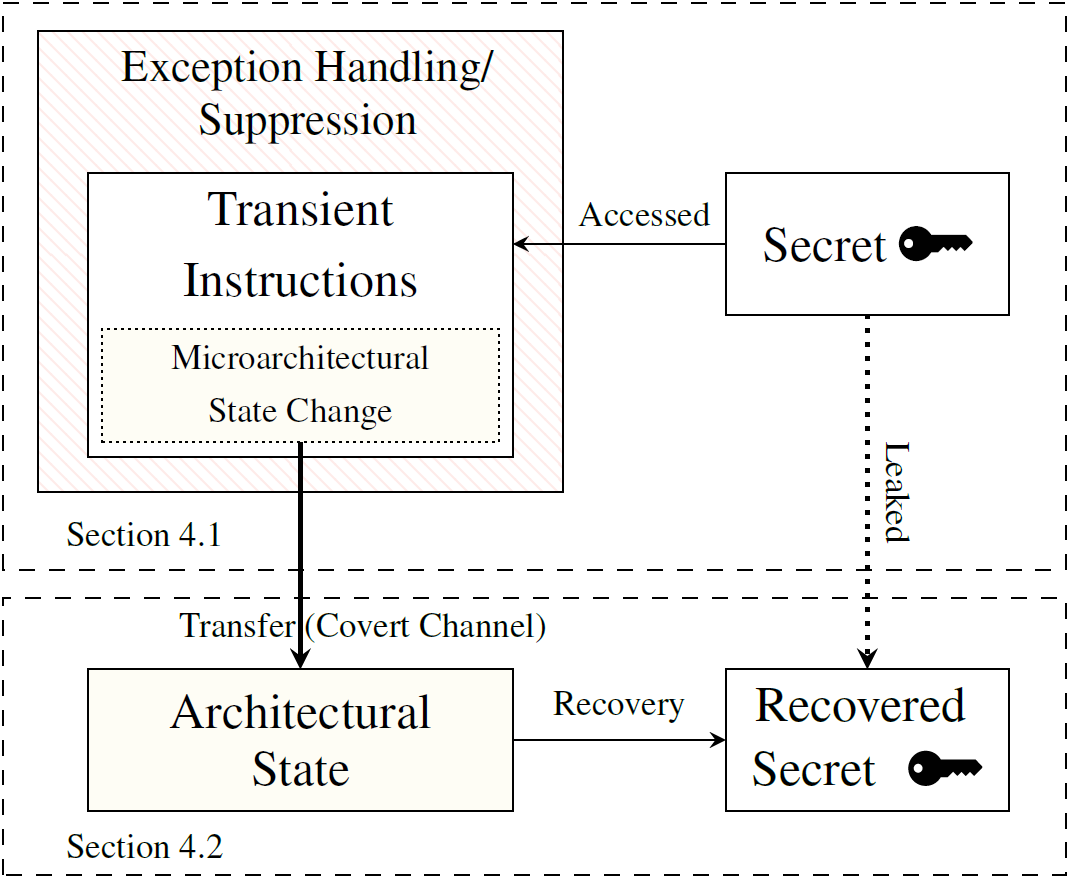
\includegraphics[width=1\textwidth]{4.png}
        \caption{Meltdown \cite{Lipp2018meltdown}.}
    \end{figure}
    Spectre induces users to speculatively perform operations that would not occur during proper program execution, and leaks the users' confidential secrets via side channels to the adversary.\\
    In detail, the attacker executes improper operations to control the processor, and then makes the CPU to do wrong speculative predictions. Through the speculative instructions, the attacker can "transfer confidential information from the victim context into a microarchitectural side channel". Finally, the attacker can recover the sensitive data also by flush+reload (or evict+reload) \cite{Kocher2018spectre}.\\
    The countermeasure is to fix the processor designs and updates instruction set architectures (ISAs) to "give hardware architects and software developers a common understanding as to what computation state CPU implementations are and are not permitted to leak" \cite{Kocher2018spectre}.
    \item Search and explain what the Dirty COW bug is.\\
    Dirty cow (CVE-2016-5195) is a local privilege escalation bug as a computer security vulnerability for the Linux kernel that exploits a race condition in the copy-on-write mechanism \cite{dirtycowwiki}. The word "cow" is the abbreviation for "copy-on-write" or "change on write".\\
    To elaborate this problem, consider two variables \texttt{a = 'COW'} and \texttt{b = a}, both of them are pointed at the same memory object. Then, the operating system waits until the value of \texttt{b} is actually modified, supposing that we do \texttt{b += ' Dirty'}. Linux allocates memory for the new, modified version of the object, reads \texttt{'COW'}, appends \texttt{' Dirty'}, and writes the modified contents into the newly allocated area of memory.\\
    The race condition between reading \texttt{'COW'} and writing modified contents into memory of \texttt{b} will trick the memory mapper to write modified contents into the original memory range like the memory of \texttt{a} \cite{dirtycow}.\\
    An attacker can use the race condition to bypass a framework called discretionary access controls (DAC) of Linux. A carefully "crafted attack can indeed replace "/bin/bash" with a malicious version by an unprivileged user" \cite{dirtycow}.\\
    Nowadays, many Linux distributions have published fixes to solve this bug, like SUSE.
\end{enumerate}
\section*{Ex. 4 — Linux}
Write a very short C program that leads to thrashing.
\inputminted[frame=single,bgcolor=bg,breaklines,linenos]{c}{h6ex4.c}
\begin{figure}[H]
    \centering
    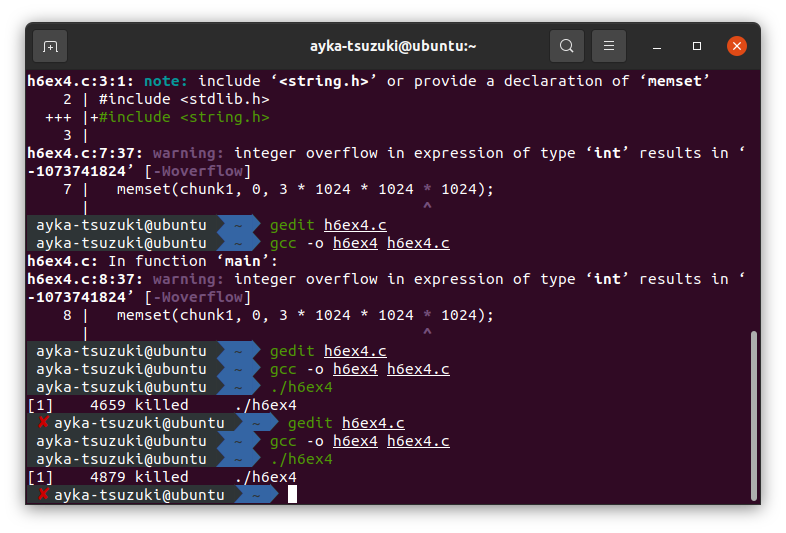
\includegraphics[width=1\textwidth]{1.png}
    \caption{Thrashing.}
\end{figure}
This program works on my VMware station Ubuntu virtual machine with 3 GiB memory. By using \texttt{htop} command, we can see that the memory of the program reaches to almost 100\% at the peak.
\printbibliography
\end{document}